\documentclass[12pt,a4paper,openany]{article}

\usepackage{array}
\newcolumntype{C}{>{\centering\arraybackslash}p{9.6em}}

\usepackage{fontspec}
\usepackage{epigraph}
\usepackage{polyglossia}
\setdefaultlanguage{english}
\setotherlanguage[variant=ancient]{greek}
\setotherlanguage{french}
\setotherlanguage{russian}
\setlength{\epigraphwidth}{24em}

\usepackage{longtable}
\newcolumntype{B}[1]{>{\large\bfseries}c{#1}}
\newcolumntype{T}[1]{>{\ttfamily}l{#1}}
\usepackage{rotating}

\defaultfontfeatures{Ligatures=TeX}
\setmainfont{OldStandardTT-Regular}
%\setmainfont[  ItalicFont={Linux Libertine Italic},
%                BoldFont={Linux Libertine Bold}]{TheanoOldStyle-Regular}

\hoffset=-1in
\voffset=-1in
\oddsidemargin=30mm
\evensidemargin=20mm
\textwidth=160mm
\textheight=228mm

\catcode"2019=12
\lccode"2019="2019

\usepackage{array}

\usepackage{fancyhdr}
\setlength{\topmargin}{48pt}
\setlength{\headheight}{32pt}
\setlength{\headsep}{16pt}
\renewcommand{\headrulewidth}{0.5pt}
\newcommand{\pageheader}[1]{%
	\clearpage
	\pagestyle{fancy}
	\lhead{\LARGE\bfseries#1}
	\cfoot{}
}

\newenvironment{samples}[1]{
        \oddsidemargin=42.7mm
        \fontspec{#1}
}{}
\newcommand{\sampletitle}[1]{%
        \addvspace{\bigskipamount}
        \noindent#1
        \smallskip
}
\newcommand{\sampleheader}[1]{%
	\addvspace{1.2\bigskipamount}
	\vbox{\noindent{\large\bfseries#1}\par
	\vskip 4pt
	\noindent\hrule width \textwidth height 0.5pt
	\vskip-.5pt}
	\smallskip
}

\makeatletter
\newcommand\featuretitle{\@startsection {section}{1}{\z@}%
        {-18pt plus -6pt minus -12pt}%
        {12pt plus 4pt minus 8pt}%
        {\normalfont\Large\bfseries}
}
\makeatother

\begin{document}

\pagestyle{empty}
\mbox{}

\vspace{\stretch{0.1}}

\centerline{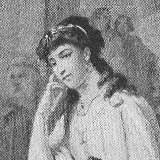
\includegraphics[width=56mm]{theano160.png}}

\vspace{\stretch{0.2}}

\centerline{\fontspec{TheanoOldStyle-Regular}\fontsize{48}{56}\selectfont ΘΕΑΝΩ}
\medskip

\centerline{\fontspec{TheanoOldStyle-Regular}\fontsize{48}{56}\selectfont Classical Fonts}

\bigskip

\rule{\textwidth}{0.5pt}

\bigskip

\centerline{\Large\itshape Type Specimen}

\bigskip

\rule{\textwidth}{0.5pt}

\vspace{\stretch{1}}

\centerline{\Large by Alexey Kryukov}

\vspace{\stretch{0.6}}

\centerline{Copyright © 2007--2008, Alexey Kryukov}

\pageheader{Theano Classical Fonts}

\epigraph{
\fontspec{TheanoModern-Regular}
Ἡσυχίης τόδ᾽ ἄθυρμ᾽ ἐμὸν ἠδέ τε λέσχη μακρὰ\\
ἀνδρὸς ἀκηδιόωντος ἀήματι νυσταλόεντι,\\
οὐ μὰν ἄμουσον πάμπαν ὅλον τὸ πόνημα πέπαικται,\\
ἀλλ᾽ ἐπιμὶξ τῆς παιδιῆς ἔσθ᾽ ἃ καὶ ἐσπούδασται.\\
Οὐδέ γε αὖ ἱερῇ πολιῇ καθάπαξ ἀπεοικὸς\\
οὔνομα καὶ Θεανὼ κικλίσκεται, οὔνομα σεμνόν\\
καί κε σὺ τοῦτο γνώσεαι, ὦ φίλος, αὐτίκ᾽ ἐπελθών.
}{Michael Choniates, metropolit of Athens\\ (ca. 1212)}

Theano is a common name for some fonts I have designed from historic
samples. Most of these fonts were initially intended as Greek-only
faces, but finally I found it interesting to supplement them with
stylistically compatible Latin letters, thus reproducing the general
look of old classical text editions. For this reason Theano fonts currently
have no additional weights or styles and don't provide extensive Unicode
coverage: just a standard set of Latin and Greek characters (including
the~full polytonic set) and some additional characters I found interesting
to~design. Nevertheless I decided to make them publicly available in the
hope they can be useful for other classicists or medievalists.

The package is named after Theano, a famous Ancient Greek woman
philosopher, who was first a student of Pythagoras, and supposedly became
his wife. In 1211 or 1212 Michael Choniates, a highly educated Greek
Metropolitan of Athens, wrote a large poem devoted to Theano (the προοίμιον
of that poem is used as an epigraph for this document). Thus Theano seemed a
good example of a person joining the ancient and the medieval world.
Another reason for which I selected her name is that it starts from
\textit{theta}, just like Thessalonica (Θεσσαλονίκη in Greek)~--- the
name of my keyboard input and conversion utility for Ancient Greek.

The package currently includes the following fonts:

\begin{description}

\item[Theano Didot] A classicist face, with both its Roman and Greek
parts implemented in Didot style. Unlike Old Standard, this font is
designed from French sources.

\item[Theano Modern] A font with Greek letters designed in the Porsonic
style. Unlike most modern implementation, it is based on Figgins Pica
No.\,3~/ Small Pica No.\,2~--- probably the most successful and once the most
popular Greek face of a Porsonic origin\footnote{See about this face
\textit{John H.~Bowman}, Greek Printing Types in Britain from the late
eighteenth to the early twentieth century. \textit{Typophilia}, 1998.
P.~127--128. The author calls this type ``the most beattiful Greek type
ever devised.''}~--- rather than on later Monotype's design. The accompanying
Latin font is implemented in the Modern style and modelled after English
Modern faces of later 19\textsuperscript{th} century, often used alonglide
with Porsonic Greek types.

\item[Theano Old Style] A modernized ``Old Style'' Greek font with a large
number of historical ligatures and alternate forms, modelled after some early
19\textsuperscript{th} century types designed by Figgins' type foundry. It
is accompanied by a Latin face based on some ``Old Style'' Roman fonts of the
late 19\textsuperscript{th} and early 20\textsuperscript{th} century.

\end{description}

\pageheader{Theano Didot~--- Roman Characters}

\hspace\parindent\begin{minipage}[t]{\dimexpr\textwidth-\parindent\relax}
\fontspec{TheanoDidot-Regular}

\sampletitle{Theano Didot Regular 10 pt}

{\fontsize{10}{12}\selectfont\noindent
Voyez le brick géant que j’examine près du wharf.\\
Falsches Üben von Xylophonmusik quält jeden größeren Zwerg.\\
Kæmi ný öxi hér ykist þjófum nú bæði víl og ádrepa.\\
ABCDEFGHIJKLMNOPQRSTUVWXYZ \$0123456789
}

\sampletitle{Theano Didot Regular 12 pt}

{\fontsize{12}{14}\selectfont\noindent
Voyez le brick géant que j’examine près du wharf.\\
Falsches Üben von Xylophonmusik quält jeden größeren Zwerg.\\
Kæmi ný öxi hér ykist þjófum nú bæði víl og ádrepa.\\
ABCDEFGHIJKLMNOPQRSTUVWXYZ \$0123456789
}

\sampletitle{Theano Didot Regular 14 pt}

{\fontsize{14}{18}\selectfont\noindent
Voyez le brick géant que j’examine près du wharf.\\
Falsches Üben von Xylophonmusik quält jeden größeren Zwerg.\\
Kæmi ný öxi hér ykist þjófum nú bæði víl og ádrepa.\\
ABCDEFGHIJKLMNOPQRSTUVWXYZ \$0123456789
}

\sampletitle{Theano Didot Regular 16 pt}

{\fontsize{16}{20}\selectfont\noindent
Voyez le brick géant que j’examine près du wharf.\\
Falsches Üben von Xylophonmusik quält jeden größeren Z\\
Kæmi ný öxi hér ykist þjófum nú bæði víl og ádrepa.\\
ABCDEFGHIJKLMNOPQRSTUVWXYZ \$0123456789
}
\end{minipage}

\vfill
\vspace{-\smallskipamount}

\sampleheader{Sample text at 14 pt}

\begin{otherlanguage}{french}
\parfillskip=0pt
\fontspec{TheanoDidot-Regular}\fontsize{14}{18}\selectfont

\noindent Poussés par ces motifs et entraînés par l’ascendant d’Orgétorix,
ils commencent à tout disposer pour le départ, rassemblent un grand nombre
de bêtes de somme et de chariots, ensemencent toutes leurs terres, afin de
s’assurer des vivres dans leur marche et renouvellent avec leurs voisins les
traités de paix et d’alliance. Ils pensèrent que deux ans leur suffiraient
pour ces préparatifs; et une loi fixa le départ à la troisième année.
Orgétorix est choisi pour présider à l’entreprise. Envoyé en qualité
de~député vers les cités voisines, sur sa route, il engage le Séquanais
Casticos, fils de Catamantaloédis, et dont le père avait longtemps régné en
Séquanie et avait reçu du peuple romain le titre d’ami, à reprendre sur
ses concitoyens l’autorité suprême, précédemment exercée par son père.
Il inspire le même dessein à l’Héduen Dumnorix, frère de Diviciacos, qui
tenait alors le premier rang dans la cité et était très aimé du peuple;
il lui donne sa fille en mariage. Il leur démontre la facilité du succès
de leurs efforts; devant lui-même s’em-

\end{otherlanguage}

\pageheader{Theano Didot~--- Cyrillic Characters}

\hspace\parindent\begin{minipage}[t]{\dimexpr\textwidth-\parindent\relax}
\fontspec{TheanoDidot-Regular}

\sampletitle{Theano Didot Regular 10 pt}

{\fontsize{10}{12}\selectfont\noindent
На душномъ фонѣ лицемѣрящей эпохи ярко зажглись вѣчные абсолюты.\\
Реците жељу и биће~--- мађија џиновског духа из флаше почиње.\\
АБВГҐДЂЕЄЁЖЗИІЇЈЙКЛЉМНЊОПРСТЋУЎФХЦЧЏШЩЪЫЬѢЭЮЯѲѴ
}

\sampletitle{Theano Didot Regular 12 pt}

{\fontsize{12}{14}\selectfont\noindent
На душномъ фонѣ лицемѣрящей эпохи ярко зажглись вѣчные абсолюты.\\
Реците жељу и биће~--- мађија џиновског духа из флаше почиње.\\
АБВГҐДЂЕЄЁЖЗИІЇЈЙКЛЉМНЊОПРСТЋУЎФХЦЧЏШЩЪЫЬѢЭЮЯѲ
}

\sampletitle{Theano Didot Regular 14 pt}

{\fontsize{14}{18}\selectfont\noindent
На душномъ фонѣ лицемѣрящей эпохи ярко зажглись вѣчные абсо\\
Реците жељу и биће~--- мађија џиновског духа из флаше почиње.\\
АБВГҐДЂЕЄЁЖЗИІЇЈЙКЛЉМНЊОПРСТЋУЎФХЦЧЏШЩЪЫ
}

\sampletitle{Theano Didot Regular 16 pt}

{\fontsize{16}{20}\selectfont\noindent
На душномъ фонѣ лицемѣрящей эпохи ярко зажглись вѣч\\
Реците жељу и биће~--- мађија џиновског духа из флаше п\\
АБВГҐДЂЕЄЁЖЗИІЇЈЙКЛЉМНЊОПРСТЋУЎФХЦЧЏ
}

\end{minipage}

\vfill

\sampleheader{Sample text at 14 pt}

\begin{otherlanguage}{russian}
\parfillskip=0pt
\fontspec{TheanoDidot-Regular}\fontsize{14}{18}\selectfont

\noindent Въ последовавшей за тѣмъ битве пострадалъ центръ аѳинскаго
войска. Здесь противъ Леонтійской и Антіохійской фѵлъ непріятель
защищался особенно долго и упорно. Ѳемистоклъ и Аристидъ, находясь на
одной боевой линіи другъ подлѣ друга, вступили въ славное соперничество,
ибо одинъ принадлежалъ къ Леонтійской фѵле, а другой къ Антіохійской.
Аѳиняне обратили варваровъ въ бегство и отбросили ихъ къ кораблямъ. Замѣтивъ
однако, что флотъ непріятельскій не направился къ островамъ, но противъ
воли пригонялся вѣтромъ и водою къ берегамъ Аттики, они стали опасаться,
чтобы городъ не былъ настигнутъ въ расплохъ. Поэтому девять фѵлъ тотчасъ
же двинулись поспѣшнымъ маршемъ къ Аѳинамъ и прибыли туда въ тотъ же день;
а Аристидъ съ своею фѵлою остался въ Мараѳонѣ для охраненія плѣнныхъ и
военной добычи. И въ этомъ случаѣ онъ выполнилъ съ честію возложенныя на
него надежды. Повсюду разсыпаны были золото и серебро; въ палаткахъ и на
захваченныхъ корабляхъ лежали грудами разныя платья и другія драгоцѣнныя
вещи. Аристидъ самъ не польстился на нихъ и другимъ не даль до нихъ
дотронуться, кромѣ тѣхъ немногихъ, которые успѣли тайкомъ

\end{otherlanguage}

\pageheader{Theano Didot~--- Greek Characters}

\hspace\parindent\begin{minipage}[t]{\dimexpr\textwidth-\parindent\relax}
\fontspec{TheanoDidot-Regular}

\sampletitle{Theano Didot Regular 10 pt}

{\fontsize{10}{12}\selectfont\noindent
Ζαφείρι δέξου πάγκαλο, βαθῶν ψυχῆς τὸ σῆμα. ϐϑϕϱϲ\\
Ἐξ ὧν γραφὴν γραψάμενος καὶ ἐμὲ διαβάλλων ἐλπίζει χρήματα λήψεσθαι.\\
ΑΒΓΔΕΖΗΘϴΙΚΛΜΝΞΟΠΡΣΤΥΦΧΨΩ ϘϙϚϛϜϝϞϟϠϡ
}

\sampletitle{Theano Didot Regular 12 pt}

{\fontsize{12}{14}\selectfont\noindent
Ζαφείρι δέξου πάγκαλο, βαθῶν ψυχῆς τὸ σῆμα. ϐϑϕϱϲ\\
Ἐξ ὧν γραφὴν γραψάμενος καὶ ἐμὲ διαβάλλων ἐλπίζει χρήματα λήψεσθαι.\\
ΑΒΓΔΕΖΗΘϴΙΚΛΜΝΞΟΠΡΣΤΥΦΧΨΩ ϘϙϚϛϜϝϞϟϠϡ
}

\sampletitle{Theano Didot Regular 14 pt}

{\fontsize{14}{18}\selectfont\noindent
Ζαφείρι δέξου πάγκαλο, βαθῶν ψυχῆς τὸ σῆμα. ϐϑϕϱϲ\\
Ἐξ ὧν γραφὴν γραψάμενος καὶ ἐμὲ διαβάλλων ἐλπίζει χρήματα λήψε\\
ΑΒΓΔΕΖΗΘϴΙΚΛΜΝΞΟΠΡΣΤΥΦΧΨΩ ϘϙϚϛϜϝϞϟϠϡ
}

\sampletitle{Theano Didot Regular 16 pt}

{\fontsize{16}{20}\selectfont\noindent
Ζαφείρι δέξου πάγκαλο, βαθῶν ψυχῆς τὸ σῆμα. ϐϑϕϱϲ\\
Ἐξ ὧν γραφὴν γραψάμενος καὶ ἐμὲ διαβάλλων ἐλπίζει χρήμα\\
ΑΒΓΔΕΖΗΘϴΙΚΛΜΝΞΟΠΡΣΤΥΦΧΨΩ ϘϙϚϛϜϝϞϟϠϡ
}

\end{minipage}

\vfill

\sampleheader{Sample text at 14 pt}

\begin{otherlanguage}{greek}
\parfillskip=0pt
\fontspec[RawFeature=+calt]{TheanoDidot-Regular}\fontsize{14}{18}\selectfont

\noindent Ἄνδρες στρατιῶται, μὴ θαυμάζετε ὅτι χαλεπῶς φέρω
τοῖς παροῦσι πράγμασιν.  ἐμοὶ γὰρ ξένος Κῦρος ἐγένετο καί με φεύγοντα ἐκ
τῆς πατρίδος τά τε ἄλλα ἐτίμησε καὶ μυρίους ἔδωκε δαρεικούς· οὓς ἐγὼ λαβὼν
οὐκ εἰς τὸ ἴδιον κατεθέμην ἐμοὶ οὐδὲ καθ\-ηδυπάθησα, ἀλλ᾽ εἰς ὑμᾶς ἐδαπάνων.
[1.3.4] καὶ πρῶτον μὲν πρὸς τοὺς Θρᾷκας ἐπολέμησα, καὶ ὑπὲρ τῆς Ἑλλάδος
ἐτιμωρούμην μεθ᾽ ὑμῶν, ἐκ τῆς Χεῤῥονήσου αὐτοὺς ἐξελαύνων βουλομένους
ἀφαιρεῖσθαι τοὺς ἐνοικοῦντας Ἕλληνας τὴν γῆν. ἐπειδὴ δὲ Κῦρος ἐκάλει, λαβὼν
ὑμᾶς ἐπορευόμην, ἵνα εἴ τι δέοιτο ὠφελοίην αὐτὸν ἀνθ᾽ ὧν εὖ ἔπαθον ὑπ᾽
ἐκείνου. [1.3.5] ἐπεὶ δὲ ὑμεῖς οὐ βούλεσθε συμπορεύεσθαι, ἀνάγκη δή μοι ἢ
ὑμᾶς προδόντα τῇ Κύρου φιλίᾳ χρῆσθαι ἢ πρὸς ἐκεῖνον ψευσάμενον μεθ᾽ ὑμῶν
εἶναι.  εἰ μὲν δὴ δίκαια ποιήσω οὐκ οἶδα, αἱρήσομαι δ᾽ οὖν ὑμᾶς καὶ σὺν
ὑμῖν ὅ τι ἂν δέῃ πείσομαι.  καὶ οὔποτε ἐρεῖ οὐδεὶς ὡς ἐγὼ Ἕλληνας ἀγαγὼν
εἰς τοὺς βαρβάρους, προδοὺς τοὺς Ἕλληνας τὴν τῶν βαρβάρων φιλίαν εἱλόμην,
[1.3.6] ἀλλ᾽ ἐπεὶ ὑμεῖς ἐμοὶ οὐ θέλετε πείθεσθαι, ἐγὼ σὺν ὑμῖν ἕψομαι καὶ ὅ
τι ἂν δέῃ πείσομαι. νομίζω γὰρ ὑμᾶς ἐμοὶ εἶναι καὶ πατρίδα καὶ φίλους καὶ
συμμάχους, καὶ σὺν ὑμῖν μὲν ἂν οἶμαι εἶναι τίμιος ὅπου ἂν ὦ, ὑμῶν δὲ
ἔρημος ὢν οὐκ ἂν ἱκανὸς οἶμαι εἶναι οὔτ᾽ ἂν φίλον ὠφελῆσαι οὔτ᾽ ἂν ἐχθρὸν
ἀλέξασθαι. ὡς ἐμοῦ οὖν ἰόντος ὅπῃ ἂν καὶ ὑμεῖς οὕτω τὴν γνώμην ἔχετε.
[1.3.7] ταῦτα εἶπεν· οἱ

\end{otherlanguage}

\pageheader{Theano Didot~--- Smart Font Features}

\featuretitle*{Old Style Numerals}

\begin{center}
\LARGE
\begin{tabular}[c]{ccc}

\fontspec[Script=Latin,Color=696969]{TheanoDidot-Regular}
0123456789 & ⇒ &
\fontspec[Script=Latin,RawFeature=+onum]{TheanoDidot-Regular}
0123456789 \\

\end{tabular}
\end{center}

\featuretitle*{Diagonal Fractions}

\begin{center}
\LARGE
\begin{tabular}[c]{ccc}

\fontspec[Script=Latin,Color=696969]{TheanoDidot-Regular}
{1/4} {1/2} {3/4}  & ⇒ &
\fontspec[Script=Latin,RawFeature=+frac]{TheanoDidot-Regular}
{1/4} {1/2} {3/4} \\

\end{tabular}
\end{center}

\featuretitle*{Common Ligatures}

\begin{center}
\LARGE
\begin{tabular}[c]{ccc}

\fontspec[Script=Latin,Color=696969,RawFeature=-liga]{TheanoDidot-Regular}
flamma fidei efficacis  & ⇒ &
\fontspec[Script=Latin]{TheanoDidot-Regular}
flamma fidei efficacis \\

\end{tabular}
\end{center}

\featuretitle*{Localized Forms for Romanian and Stylistic Set 01}

\begin{center}
\LARGE
\begin{tabular}[c]{ccc}

\fontspec[Script=Latin,Color=696969]{TheanoDidot-Regular}
raţiune şi conştiinţă & ⇒ &
\fontspec[Script=Latin,Language=Romanian]{TheanoDidot-Regular}
raţiune şi conştiinţă \\

\end{tabular}
\end{center}

\featuretitle*{Combining Mark Positioning for Greek}

\begin{center}
\LARGE
\begin{tabular}[c]{ccc}

\fontspec[Script=Greek,Color=696969]{TheanoDidot-Regular}
τα◌͂ς Θεο◌̄◌͂ ε◌̄◌̓◌́ναι & ⇒ &
\fontspec[Script=Greek]{TheanoDidot-Regular}
τᾶς θεο̄͂ ε̄̓́ναι \\

\end{tabular}
\end{center}

\featuretitle*{Contextual Alternates}

Theano Didot provides a contextual substitution rule allowing to
substitute a medial/final form for the Greek \textit{beta}
at the appropriate places. This rule should be active by default
in most applications which support it, as it is required by French
rules of Greek typesetting.

\begin{center}
\LARGE
\begin{tabular}[c]{ccc}

\fontspec[Script=Greek,Color=696969]{TheanoDidot-Regular}
βαβαὶ τοῦ βαρβαρισμοῦ & ⇒ &
\fontspec[Script=Greek,RawFeature=+calt]{TheanoDidot-Regular}
βαβαὶ τοῦ βαρβαρισμοῦ \\

\end{tabular}
\end{center}

\featuretitle*{Stylistic Set 11}

When used in combination with contextual alternates, this stylistic
set causes initial and final/medial forms of \textit{theta} to be
differentiated. Otherwise it just replaces the default ‟closed” glyph
for \textit{theta} with the ‟script” form.

\begin{center}
\LARGE
\begin{tabular}[c]{ccc}

\fontspec[Script=Greek,RawFeature={+calt;Color=696969}]{TheanoDidot-Regular}
θαυμασθεὶς βάρβαρος & ⇒ &
\fontspec[Script=Greek,RawFeature={+ss11;+calt}]{TheanoDidot-Regular}
θαυμασθεὶς βάρβαρος \\

\end{tabular}
\end{center}

\pageheader{Theano Modern~--- Roman Characters}

\hspace\parindent\begin{minipage}[t]{\dimexpr\textwidth-\parindent\relax}
\fontspec{TheanoModern-Regular}

\sampletitle{Theano Modern Regular 10 pt}

{\fontsize{10}{12}\selectfont\noindent
A quick brown fox jumps over the lazy dog.\\
Falsches Üben von Xylophonmusik quält jeden größeren Zwerg.\\
Kæmi ný öxi hér ykist þjófum nú bæði víl og ádrepa.\\
ABCDEFGHIJKLMNOPQRSTUVWXYZ \$0123456789
}

\sampletitle{Theano Modern Regular 12 pt}

{\fontsize{12}{14}\selectfont\noindent
A quick brown fox jumps over the lazy dog.\\
Falsches Üben von Xylophonmusik quält jeden größeren Zwerg.\\
Kæmi ný öxi hér ykist þjófum nú bæði víl og ádrepa.\\
ABCDEFGHIJKLMNOPQRSTUVWXYZ \$0123456789
}

\sampletitle{Theano Modern Regular 14 pt}

{\fontsize{14}{18}\selectfont\noindent
A quick brown fox jumps over the lazy dog.\\
Falsches Üben von Xylophonmusik quält jeden größeren Zwerg.\\
Kæmi ný öxi hér ykist þjófum nú bæði víl og ádrepa.\\
ABCDEFGHIJKLMNOPQRSTUVWXYZ \$0123456789
}

\sampletitle{Theano Modern Regular 16 pt}

{\fontsize{16}{20}\selectfont\noindent
A quick brown fox jumps over the lazy dog.\\
Falsches Üben von Xylophonmusik quält jeden größeren Z\\
Kæmi ný öxi hér ykist þjófum nú bæði víl og ádrepa.\\
ABCDEFGHIJKLMNOPQRSTUVWXYZ \$0123456789
}
\end{minipage}

\vfill

\sampleheader{Sample text at 14 pt}

\begin{otherlanguage}{english}
\parfillskip=0pt
\fontspec{TheanoModern-Regular}\fontsize{14}{18}\selectfont

\noindent Induced by these considerations, and influenced by the authority
of Orgetorix, they determined to provide such things as were necessary for
their expedition — to buy up as great a number as possible of beasts of
burden and wagons — to make their sowings as large as possible, so that on
their march plenty of corn might be in store — and to establish peace and
friendship with the neighboring states. They reckoned that a term of two
years would be sufficient for them to execute their designs; they fix by
decree their departure for the third year. Orgetorix is chosen to complete
these arrangements. He took upon himself the office of embassador to the
states: on this journey he persuades Casticus, the son of Catamantaledes
(one of the Sequani, whose father had possessed the sovereignty among the
people for many years, and had been styled “friend” by the senate of the
Roman people), to seize upon the sovereignty in his own state, which his
father had held before him, and he likewise persuades Dumnorix, an Æduan,
the brother

\end{otherlanguage}

\pageheader{Theano Modern~--- Cyrillic Characters}

\hspace\parindent\begin{minipage}[t]{\dimexpr\textwidth-\parindent\relax}
\fontspec{TheanoModern-Regular}

\sampletitle{Theano Modern Regular 10 pt}

{\fontsize{10}{12}\selectfont\noindent
На душномъ фонѣ лицемѣрящей эпохи ярко зажглись вѣчные абсолюты.\\
Реците жељу и биће~--- мађија џиновског духа из флаше почиње.\\
АБВГҐДЂЕЄЁЖЗИІЇЈЙКЛЉМНЊОПРСТЋУЎФХЦЧЏШЩЪЫЬѢЭЮЯѲѴ
}

\sampletitle{Theano Modern Regular 12 pt}

{\fontsize{12}{14}\selectfont\noindent
На душномъ фонѣ лицемѣрящей эпохи ярко зажглись вѣчные абсолюты.\\
Реците жељу и биће~--- мађија џиновског духа из флаше почиње.\\
АБВГҐДЂЕЄЁЖЗИІЇЈЙКЛЉМНЊОПРСТЋУЎФХЦЧЏШЩЪЫЬѢЭЮ
}

\sampletitle{Theano Modern Regular 14 pt}

{\fontsize{14}{18}\selectfont\noindent
На душномъ фонѣ лицемѣрящей эпохи ярко зажглись вѣчные абс\\
Реците жељу и биће~--- мађија џиновског духа из флаше почиње.\\
АБВГҐДЂЕЄЁЖЗИІЇЈЙКЛЉМНЊОПРСТЋУЎФХЦЧЏШЩ
}

\sampletitle{Theano Modern Regular 16 pt}

{\fontsize{16}{20}\selectfont\noindent
На душномъ фонѣ лицемѣрящей эпохи ярко зажглись вѣ\\
Реците жељу и биће~--- мађија џиновског духа из флаше п\\
АБВГҐДЂЕЄЁЖЗИІЇЈЙКЛЉМНЊОПРСТЋУЎФХЦЧ
}

\end{minipage}

\vfill

\sampleheader{Sample text at 14 pt}

\begin{otherlanguage}{russian}
\parfillskip=0pt
\fontspec{TheanoModern-Regular}\fontsize{14}{18}\selectfont

\noindent Въ последовавшей за тѣмъ битве пострадалъ центръ аѳинскаго
войска. Здесь противъ Леонтійской и Антіохійской фѵлъ непріятель
защищался особенно долго и упорно. Ѳемистоклъ и Аристидъ, находясь на
одной боевой линіи другъ подлѣ друга, вступили въ славное соперничество,
ибо одинъ принадлежалъ къ Леонтійской фѵле, а другой къ Антіохійской.
Аѳиняне обратили варваровъ въ бегство и отбросили ихъ къ кораблямъ. Замѣтивъ
однако, что флотъ непріятельскій не направился къ островамъ, но противъ
воли пригонялся вѣтромъ и водою къ берегамъ Аттики, они стали опасаться,
чтобы городъ не былъ настигнутъ въ расплохъ. Поэтому девять фѵлъ тотчасъ
же двинулись поспѣшнымъ маршемъ къ Аѳинамъ и прибыли туда въ тотъ же день;
а Аристидъ съ своею фѵлою остался въ Мараѳонѣ для охраненія плѣнныхъ и
военной добычи. И въ этомъ случаѣ онъ выполнилъ съ честію возложенныя на
него надежды. Повсюду разсыпаны были золото и серебро; въ палаткахъ и на
захваченныхъ корабляхъ лежали грудами разныя платья и другія драгоцѣнныя
вещи. Аристидъ самъ не польстился на нихъ и другимъ не даль до нихъ
дотронуться, кромѣ тѣхъ немногихъ, которые успѣли тайкомъ

\end{otherlanguage}

\pageheader{Theano Modern~--- Greek Characters}

\hspace\parindent\begin{minipage}[t]{\dimexpr\textwidth-\parindent\relax}
\fontspec{TheanoModern-Regular}

\sampletitle{Theano Modern Regular 10 pt}

{\fontsize{10}{12}\selectfont\noindent
Ζαφείρι δέξου πάγκαλο, βαθῶν ψυχῆς τὸ σῆμα. ϐϑϰϱϲ\\
Ἐξ ὧν γραφὴν γραψάμενος καὶ ἐμὲ διαβάλλων ἐλπίζει χρήματα λήψεσθαι.\\
ΑΒΓΔΕΖΗΘϴΙΚΛΜΝΞΟΠΡΣΤΥϒΦΧΨΩ ϘϙϚϛϜϝϞϟϠϡ
}

\sampletitle{Theano Modern Regular 12 pt}

{\fontsize{12}{14}\selectfont\noindent
Ζαφείρι δέξου πάγκαλο, βαθῶν ψυχῆς τὸ σῆμα. ϐϑϰϱϲ\\
Ἐξ ὧν γραφὴν γραψάμενος καὶ ἐμὲ διαβάλλων ἐλπίζει χρήματα λήψεσθαι.\\
ΑΒΓΔΕΖΗΘϴΙΚΛΜΝΞΟΠΡΣΤΥϒΦΧΨΩ ϘϙϚϛϜϝϞϟϠϡ
}

\sampletitle{Theano Modern Regular 14 pt}

{\fontsize{14}{18}\selectfont\noindent
Ζαφείρι δέξου πάγκαλο, βαθῶν ψυχῆς τὸ σῆμα. ϐϑϰϱϲ\\
Ἐξ ὧν γραφὴν γραψάμενος καὶ ἐμὲ διαβάλλων ἐλπίζει χρήματα λήψε\\
ΑΒΓΔΕΖΗΘϴΙΚΛΜΝΞΟΠΡΣΤΥϒΦΧΨΩ ϘϙϚϛϜϝϞϟϠϡ
}

\sampletitle{Theano Modern Regular 16 pt}

{\fontsize{16}{20}\selectfont\noindent
Ζαφείρι δέξου πάγκαλο, βαθῶν ψυχῆς τὸ σῆμα. ϐϑϰϱϲ\\
Ἐξ ὧν γραφὴν γραψάμενος καὶ ἐμὲ διαβάλλων ἐλπίζει χρημ\\
ΑΒΓΔΕΖΗΘϴΙΚΛΜΝΞΟΠΡΣΤΥϒΦΧΨΩ ϘϙϚϛϜϝϞϟϠϡ
}

\end{minipage}

\vfill

\sampleheader{Sample text at 14 pt}

\begin{otherlanguage}{greek}
\fontspec{TheanoModern-Regular}\fontsize{14}{18}\selectfont

\parfillskip=0pt\noindent Ἄνδρες στρατιῶται, μὴ θαυμάζετε ὅτι χαλεπῶς φέρω
τοῖς παροῦσι πράγμασιν.  ἐμοὶ γὰρ ξένος Κῦρος ἐγένετο καί με φεύγοντα ἐκ
τῆς πατρίδος τά τε ἄλλα ἐτίμησε καὶ μυρίους ἔδωκε δαρεικούς· οὓς ἐγὼ λαβὼν
οὐκ εἰς τὸ ἴδιον κατεθέμην ἐμοὶ οὐδὲ καθηδυπάθησα, ἀλλ᾽ εἰς ὑμᾶς ἐδαπάνων.
[1.3.4] καὶ πρῶτον μὲν πρὸς τοὺς Θρᾷκας ἐπολέμησα, καὶ ὑπὲρ τῆς Ἑλλάδος
ἐτιμωρούμην μεθ᾽ ὑμῶν, ἐκ τῆς Χεῤῥονήσου αὐτοὺς ἐξελαύνων βουλομένους
ἀφαιρεῖσθαι τοὺς ἐνοικοῦντας Ἕλληνας τὴν γῆν. ἐπειδὴ δὲ Κῦρος ἐκάλει, λαβὼν
ὑμᾶς ἐπορευόμην, ἵνα εἴ τι δέοιτο ὠφελοίην αὐτὸν ἀνθ᾽ ὧν εὖ ἔπαθον ὑπ᾽
ἐκείνου.  [1.3.5] ἐπεὶ δὲ ὑμεῖς οὐ βούλεσθε συμπορεύεσθαι, ἀνάγκη δή μοι ἢ
ὑμᾶς προδόντα τῇ Κύρου φιλίᾳ χρῆσθαι ἢ πρὸς ἐκεῖνον ψευσάμενον μεθ᾽ ὑμῶν
εἶναι.  εἰ μὲν δὴ δίκαια ποιήσω οὐκ οἶδα, αἱρήσομαι δ᾽ οὖν ὑμᾶς καὶ σὺν
ὑμῖν ὅ τι ἂν δέῃ πείσομαι.  καὶ οὔποτε ἐρεῖ οὐδεὶς ὡς ἐγὼ Ἕλληνας ἀγαγὼν
εἰς τοὺς βαρβάρους, προδοὺς τοὺς Ἕλλη\-νας τὴν τῶν βαρβάρων φιλίαν εἱλόμην,
[1.3.6] ἀλλ᾽ ἐπεὶ ὑμεῖς ἐμοὶ οὐ θέλετε πείθεσθαι, ἐγὼ σὺν ὑμῖν ἕψομαι καὶ ὅ
τι ἂν δέῃ πείσομαι. νομίζω γὰρ ὑμᾶς ἐμοὶ εἶναι καὶ πατρίδα καὶ φίλους καὶ
συμμάχους, καὶ σὺν ὑμῖν μὲν ἂν οἶμαι εἶναι τίμιος ὅπου ἂν ὦ, ὑμῶν δὲ
ἔρημος ὢν οὐκ ἂν ἱκανὸς οἶμαι εἶναι οὔτ᾽ ἂν φίλον ὠφελῆσαι οὔτ᾽ ἂν ἐχθρὸν
ἀλέξασθαι. ὡς ἐμοῦ οὖν ἰόντος ὅπῃ ἂν καὶ ὑμεῖς οὕτω

\end{otherlanguage}

\pageheader{Theano Modern~--- Smart Font Features}

\featuretitle*{Old Style Numerals}

\begin{center}
\LARGE
\begin{tabular}[c]{ccc}

\fontspec[Script=Latin,Color=696969]{TheanoModern-Regular}
0123456789 & ⇒ &
\fontspec[Script=Latin,RawFeature=+onum]{TheanoModern-Regular}
0123456789 \\

\end{tabular}
\end{center}

\featuretitle*{Diagonal Fractions}

\begin{center}
\LARGE
\begin{tabular}[c]{ccc}

\fontspec[Script=Latin,Color=696969]{TheanoModern-Regular}
{1/4} {1/2} {3/4}  & ⇒ &
\fontspec[Script=Latin,RawFeature=+frac]{TheanoModern-Regular}
{1/4} {1/2} {3/4} \\

\end{tabular}
\end{center}

\featuretitle*{Common Ligatures}

\begin{center}
\LARGE
\begin{tabular}[c]{ccc}

\fontspec[Script=Latin,Color=696969,RawFeature=-liga]{TheanoModern-Regular}
flamma fidei efficacis  & ⇒ &
\fontspec[Script=Latin]{TheanoModern-Regular}
flamma fidei efficacis \\

\end{tabular}
\end{center}

\featuretitle*{Localized Forms for Romanian and Stylistic Set 01}

\begin{center}
\LARGE
\begin{tabular}[c]{ccc}

\fontspec[Script=Latin,Color=696969]{TheanoModern-Regular}
raţiune şi conştiinţă & ⇒ &
\fontspec[Script=Latin,Language=Romanian]{TheanoModern-Regular}
raţiune şi conştiinţă \\

\end{tabular}
\end{center}

\featuretitle*{Combining Mark Positioning for Greek}

\begin{center}
\LARGE
\begin{tabular}[c]{ccc}

\fontspec[Script=Greek,Color=696969]{TheanoModern-Regular}
τα◌͂ς Θεο◌̄◌͂ ε◌̄◌̓◌́ναι & ⇒ &
\fontspec[Script=Greek]{TheanoModern-Regular}
τᾶς θεο̄͂ ε̄̓́ναι \\

\end{tabular}
\end{center}

\featuretitle*{Stylistic Set 07}

Enable this to get lunate \textit{sigmas} substituted in place of normal
initial/medial and final forms.

\begin{center}
\LARGE
\begin{tabular}[c]{ccc}

\fontspec[Script=Greek,Color=696969]{TheanoModern-Regular}
βασιλεῖς Σπάρτης & ⇒ &
\fontspec[Script=Greek,RawFeature=+ss07]{TheanoModern-Regular}
βασιλεῖς Σπάρτης \\

\end{tabular}
\end{center}

\featuretitle*{Stylistic Set 08}

Among other innovative letterforms which first appeared in the original
Porson type were a fully-crossed \textit{Theta} and a specific
\textit{Upsilon} staying midway between the traditional palm-branch form
and a Latin ``Y''. However these forms were not adopted by Figgins' type
foundry for their Pica No.~2 / Small Pica No.~3 faces, which, being
typically Porsonic in other aspects, preserve traditional ``Old Style''
capitals. Theano Modern follows its prototype at this point, but allows
you to make your texts look even more Porsonic by applying this stylistic
set:

\begin{center}
\LARGE
\begin{tabular}[c]{ccc}

\fontspec[Script=Greek,Color=696969]{TheanoModern-Regular}
ΘΥΜΩΘΕΙΣ Ὕπατος & ⇒ &
\fontspec[Script=Greek,RawFeature=+ss08]{TheanoModern-Regular}
ΘΥΜΩΘΕΙΣ Ὕπατος \\

\end{tabular}
\end{center}

\pageheader{Theano Modern~--- Smart Font Features}

\featuretitle*{Stylistic Set 09}

Two different designs of small final \textit{sigma} can appear
in editions set with Figgins Pica No.~2 / Small Pica No.~3: the
first version, which did not descend below the baseline, was
subsequently (around 1850) replaced with a larger form. Particularly
I find the later form more elegant (so it is used by default), but
the earlier one is accessible via this stylistic set:

\begin{center}
\LARGE
\begin{tabular}[c]{ccc}

\fontspec[Script=Greek,Color=696969]{TheanoModern-Regular}
σοφὸς ἄνθρωπος & ⇒ &
\fontspec[Script=Greek,RawFeature=+ss09]{TheanoModern-Regular}
σοφὸς ἄνθρωπος \\

\end{tabular}
\end{center}

\featuretitle*{Stylistic Set 10}

This stylistic set replaces the Porsonic lunate \textit{epsilon} with
a 8-shaped form. One would argue that this form would look out of place
in a Porsonic font, and yet it was typically used in books printed
by Spottiswoode were the Greek text was set with Figgins Small Pica
No.~3. So I considered it reasonable to allow users reproducing this
typographic peculiarity with Theano Modern.

\begin{center}
\LARGE
\begin{tabular}[c]{ccc}

\fontspec[Script=Greek,Color=696969]{TheanoModern-Regular}
ἔμψυχος ἐλευθερία & ⇒ &
\fontspec[Script=Greek,RawFeature=+ss10]{TheanoModern-Regular}
ἔμψυχος ἐλευθερία \\

\end{tabular}
\end{center}

\featuretitle*{Stylistic Set 11}

And finally a stylistic set which can be used to differentiate
initial and medial/final forms for \textit{beta} and \textit{theta}.
Again, this may look inappropriate for a Porsonic face, as in the
original Porson Greek all alternate forms were completely abolished.
Nevertheless curly \textit{beta} and script \textit{theta} can
occasionally appear in 19\textsuperscript{th} century English and
American editions were they are used basing on standard contextual rules.
In general, Figgins Pica No.~2 / Small Pica No.~3 seems to be more tolerate
to alternate forms than other Porsonic faces: this was one reason for
which I had decided to reproduce this particular implementation of the
Porsonic design.

\begin{center}
\LARGE
\begin{tabular}[c]{ccc}

\fontspec[Script=Greek,RawFeature=+ss10,Color=696969]{TheanoModern-Regular}
θαυμασθεὶς βάρβαρος & ⇒ &
\fontspec[Script=Greek,RawFeature=+ss10;+ss11;+calt]{TheanoModern-Regular}
θαυμασθεὶς βάρβαρος \\

\end{tabular}
\end{center}

\featuretitle*{Mathematical Greek}

Enabling this feature causes some Greek letters to be replaced with
alternate forms, which look less appropriate for a Porsonic design,
but correspond more strictly to the reference glyphs shown in the Unicode
code chart. This might be important for mathematical contexts, where
special meanings are often assigned to particular character variants.
The affected letters are \textit{epsilon}, \textit{phi} and also
\textit{alpha} (its porsonic form has nothing unusual by itself, but
looks very similar to a Latin italic \textit{a}, which probably makes
it a bad choice for math typesetting).

\begin{center}
\LARGE
\begin{tabular}[c]{ccc}

\fontspec[Script=Greek,Color=696969]{TheanoModern-Regular}
α + ε + φ & ⇒ &
\fontspec[Script=Greek,RawFeature=+mgrk]{TheanoModern-Regular}
α + ε + φ \\

\end{tabular}
\end{center}

\pageheader{Theano Old Style~--- Roman Characters}
\vskip-\smallskipamount

\hspace\parindent\begin{minipage}[t]{\dimexpr\textwidth-\parindent\relax}
\fontspec{TheanoOldStyle-Regular}

\sampletitle{Theano Old Style Regular 10 pt}

{\fontsize{10}{12}\selectfont\noindent
A quick brown fox jumps over the lazy dog.\\
Falsches Üben von Xylophonmusik quält jeden größeren Zwerg.\\
Kæmi ný öxi hér ykist þjófum nú bæði víl og ádrepa.\\
ABCDEFGHIJKLMNOPQRSTUVWXYZ \$0123456789
}

\sampletitle{Theano Old Style Regular 12 pt}

{\fontsize{12}{14}\selectfont\noindent
A quick brown fox jumps over the lazy dog.\\
Falsches Üben von Xylophonmusik quält jeden größeren Zwerg.\\
Kæmi ný öxi hér ykist þjófum nú bæði víl og ádrepa.\\
ABCDEFGHIJKLMNOPQRSTUVWXYZ \$0123456789
}

\sampletitle{Theano Old Style Regular 14 pt}

{\fontsize{14}{18}\selectfont\noindent
A quick brown fox jumps over the lazy dog.\\
Falsches Üben von Xylophonmusik quält jeden größeren Zwerg.\\
Kæmi ný öxi hér ykist þjófum nú bæði víl og ádrepa.\\
ABCDEFGHIJKLMNOPQRSTUVWXYZ \$0123456789
}

\sampletitle{Theano Old Style Regular 16 pt}

{\fontsize{16}{20}\selectfont\noindent
A quick brown fox jumps over the lazy dog.\\
Falsches Üben von Xylophonmusik quält jeden größeren Z\\
Kæmi ný öxi hér ykist þjófum nú bæði víl og ádrepa.\\
ABCDEFGHIJKLMNOPQRSTUVWXYZ \$0123456789
}
\end{minipage}

\vfill
\vskip-\smallskipamount

\sampleheader{Sample text at 14 pt}

\begin{otherlanguage}{english}
\parfillskip=0pt
\fontspec{TheanoOldStyle-Regular}\fontsize{14}{18}\selectfont

\noindent Induced by these considerations, and influenced by the authority
of Orgetorix, they determined to provide such things as were necessary for
their expedition — to buy up as great a number as possible of beasts of
burden and wagons — to make their sowings as large as possible, so that on
their march plenty of corn might be in store — and to establish peace and
friendship with the neighboring states. They reckoned that a term of two
years would be sufficient for them to execute their designs; they fix by
decree their departure for the third year. Orgetorix is chosen to complete
these arrangements. He took upon himself the office of embassador to the
states: on this journey he persuades Casticus, the son of Catamantaledes
(one of the Sequani, whose father had possessed the sovereignty among the
people for many years, and had been styled “friend” by the senate of the
Roman people), to seize upon the sovereignty in his own state, which his
father had held before him, and he likewise persuades Dumnorix, an Æduan,
the brother

\end{otherlanguage}

\pageheader{Theano Old Style ~--- Cyrillic Characters}

\hspace\parindent\begin{minipage}[t]{\dimexpr\textwidth-\parindent\relax}
\fontspec{TheanoOldStyle-Regular}

\sampletitle{Theano Old Style Regular 10 pt}

{\fontsize{10}{12}\selectfont\noindent
На душномъ фонѣ лицемѣрящей эпохи ярко зажглись вѣчные абсолюты.\\
Реците жељу и биће~--- мађија џиновског духа из флаше почиње.\\
АБВГҐДЂЕЄЁЖЗИІЇЈЙКЛЉМНЊОПРСТЋУЎФХЦЧЏШЩЪЫЬѢЭЮЯѲѴ
}

\sampletitle{Theano Old Style Regular 12 pt}

{\fontsize{12}{14}\selectfont\noindent
На душномъ фонѣ лицемѣрящей эпохи ярко зажглись вѣчные абсолюты.\\
Реците жељу и биће~--- мађија џиновског духа из флаше почиње.\\
АБВГҐДЂЕЄЁЖЗИІЇЈЙКЛЉМНЊОПРСТЋУЎФХЦЧЏШЩЪЫЬѢЭЮ
}

\sampletitle{Theano Old Style Regular 14 pt}

{\fontsize{14}{18}\selectfont\noindent
На душномъ фонѣ лицемѣрящей эпохи ярко зажглись вѣчные аб\\
Реците жељу и биће~--- мађија џиновског духа из флаше почиње.\\
АБВГҐДЂЕЄЁЖЗИІЇЈЙКЛЉМНЊОПРСТЋУЎФХЦЧЏШЩ
}

\sampletitle{Theano Old Style Regular 16 pt}

{\fontsize{16}{20}\selectfont\noindent
На душномъ фонѣ лицемѣрящей эпохи ярко зажглись вѣ\\
Реците жељу и биће~--- мађија џиновског духа из флаше п\\
АБВГҐДЂЕЄЁЖЗИІЇЈЙКЛЉМНЊОПРСТЋУЎФХЦЧ
}

\end{minipage}

\vfill

\sampleheader{Sample text at 14 pt}

\begin{otherlanguage}{russian}
\parfillskip=0pt
\fontspec{TheanoOldStyle-Regular}\fontsize{14}{18}\selectfont

\noindent Въ последовавшей за тѣмъ битве пострадалъ центръ аѳинскаго
войска. Здесь противъ Леонтійской и Антіохійской фѵлъ непріятель
защищался особенно долго и упорно. Ѳемистоклъ и Аристидъ, находясь на
одной боевой линіи другъ подлѣ друга, вступили въ славное соперничество,
ибо одинъ принадлежалъ къ Леонтійской фѵле, а другой къ Антіохійской.
Аѳиняне обратили варваровъ въ бегство и отбросили ихъ къ кораблямъ. Замѣтивъ
однако, что флотъ непріятельскій не направился къ островамъ, но противъ
воли пригонялся вѣтромъ и водою къ берегамъ Аттики, они стали опасаться,
чтобы городъ не былъ настигнутъ въ расплохъ. Поэтому девять фѵлъ тотчасъ
же двинулись поспѣшнымъ маршемъ къ Аѳинамъ и прибыли туда въ тотъ же день;
а Аристидъ съ своею фѵлою остался въ Мараѳонѣ для охраненія плѣнныхъ и
военной добычи. И въ этомъ случаѣ онъ выполнилъ съ честію возложенныя на
него надежды. Повсюду разсыпаны были золото и серебро; въ палаткахъ и на
захваченныхъ корабляхъ лежали грудами разныя платья и другія драгоцѣнныя
вещи. Аристидъ самъ не польстился на нихъ и другимъ не

\end{otherlanguage}

\pageheader{Theano Old Style~--- Greek Characters}

\hspace\parindent\begin{minipage}[t]{\dimexpr\textwidth-\parindent\relax}
\fontspec{TheanoOldStyle-Regular}

\sampletitle{Theano Old Style Regular 10 pt}

{\fontsize{10}{12}\selectfont\noindent
Ζαφείρι δέξου πάγκαλο, βαθῶν ψυχῆς τὸ σῆμα. ϐϑϰϱϲ\\
Ἐξ ὧν γραφὴν γραψάμενος καὶ ἐμὲ διαβάλλων ἐλπίζει χρήματα λήψεσθαι.\\
ΑΒΓΔΕΖΗΘϴΙΚΛΜΝΞΟΠΡΣΤΥΦΧΨΩ ϘϙϚϛϜϝϞϟϠϡ
}

\sampletitle{Theano Old Style Regular 12 pt}

{\fontsize{12}{14}\selectfont\noindent
Ζαφείρι δέξου πάγκαλο, βαθῶν ψυχῆς τὸ σῆμα. ϐϑϰϱϲ\\
Ἐξ ὧν γραφὴν γραψάμενος καὶ ἐμὲ διαβάλλων ἐλπίζει χρήματα λήψεσθαι.\\
ΑΒΓΔΕΖΗΘϴΙΚΛΜΝΞΟΠΡΣΤΥΦΧΨΩ ϘϙϚϛϜϝϞϟϠϡ
}

\sampletitle{Theano Old Style Regular 14 pt}

{\fontsize{14}{18}\selectfont\noindent
Ζαφείρι δέξου πάγκαλο, βαθῶν ψυχῆς τὸ σῆμα. ϐϑϰϱϲ\\
Ἐξ ὧν γραφὴν γραψάμενος καὶ ἐμὲ διαβάλλων ἐλπίζει χρήματα λήψε\\
ΑΒΓΔΕΖΗΘϴΙΚΛΜΝΞΟΠΡΣΤΥΦΧΨΩ ϘϙϚϛϜϝϞϟϠϡ
}

\sampletitle{Theano Old Style Regular 16 pt}

{\fontsize{16}{20}\selectfont\noindent
Ζαφείρι δέξου πάγκαλο, βαθῶν ψυχῆς τὸ σῆμα. ϐϑϰϱϲ\\
Ἐξ ὧν γραφὴν γραψάμενος καὶ ἐμὲ διαβάλλων ἐλπίζει χρημ\\
ΑΒΓΔΕΖΗΘϴΙΚΛΜΝΞΟΠΡΣΤΥΦΧΨΩ ϘϙϚϛϜϝϞϟϠϡ
}

\end{minipage}

\vfill

\sampleheader{Sample text at 14 pt}

\begin{otherlanguage}{greek}
\parfillskip=0pt
\fontspec[RawFeature=+calt]{TheanoOldStyle-Regular}\fontsize{14}{18}\selectfont

\noindent Ἄνδρες στρατιῶται, μὴ θαυμάζετε ὅτι χαλεπῶς φέρω
τοῖς παροῦσι πράγμασιν.  ἐμοὶ γὰρ ξένος Κῦρος ἐγένετο καί με φεύγοντα ἐκ
τῆς πατρίδος τά τε ἄλλα ἐτίμησε καὶ μυρίους ἔδωκε δαρεικούς· οὓς ἐγὼ λαβὼν
οὐκ εἰς τὸ ἴδιον κατεθέμην ἐμοὶ οὐδὲ καθ\-ηδυπάθησα, ἀλλ᾽ εἰς ὑμᾶς ἐδαπάνων.
[1.3.4] καὶ πρῶτον μὲν πρὸς τοὺς Θρᾷκας ἐπολέμησα, καὶ ὑπὲρ τῆς Ἑλλάδος
ἐτιμωρούμην μεθ᾽ ὑμῶν, ἐκ τῆς Χεῤῥονήσου αὐτοὺς ἐξελαύνων βουλομένους
ἀφαιρεῖσθαι τοὺς ἐνοικοῦντας Ἕλληνας τὴν γῆν. ἐπειδὴ δὲ Κῦρος ἐκάλει, λαβὼν
ὑμᾶς ἐπορευόμην, ἵνα εἴ τι δέοιτο ὠφελοίην αὐτὸν ἀνθ᾽ ὧν εὖ ἔπαθον ὑπ᾽
ἐκείνου.  [1.3.5] ἐπεὶ δὲ ὑμεῖς οὐ βούλεσθε συμπορεύεσθαι, ἀνάγκη δή μοι ἢ
ὑμᾶς προδόντα τῇ Κύρου φιλίᾳ χρῆσθαι ἢ πρὸς ἐκεῖνον ψευσάμενον μεθ᾽ ὑμῶν
εἶναι.  εἰ μὲν δὴ δίκαια ποιήσω οὐκ οἶδα, αἱρήσομαι δ᾽ οὖν ὑμᾶς καὶ σὺν
ὑμῖν ὅ τι ἂν δέῃ πείσομαι.  καὶ οὔποτε ἐρεῖ οὐδεὶς ὡς ἐγὼ Ἕλληνας ἀγαγὼν
εἰς τοὺς βαρβάρους, προδοὺς τοὺς Ἕλληνας τὴν τῶν βαρβάρων φιλίαν εἱλόμην,
[1.3.6] ἀλλ᾽ ἐπεὶ ὑμεῖς ἐμοὶ οὐ θέλετε πείθεσθαι, ἐγὼ σὺν ὑμῖν ἕψομαι καὶ ὅ
τι ἂν δέῃ πείσομαι. νομίζω γὰρ ὑμᾶς ἐμοὶ εἶναι καὶ πατρίδα καὶ φίλους καὶ
συμμάχους, καὶ σὺν ὑμῖν μὲν ἂν οἶμαι εἶναι τίμιος ὅπου ἂν ὦ, ὑμῶν δὲ
ἔρημος ὢν οὐκ ἂν ἱκανὸς οἶμαι εἶναι οὔτ᾽ ἂν φίλον ὠφελῆσαι οὔτ᾽ ἂν ἐχθρὸν
ἀλέξασθαι. ὡς ἐμοῦ οὖν ἰόντος ὅπῃ ἂν καὶ ὑμεῖς οὕτω τὴν γνώμην ἔχετε.
[1.3.7] ταῦτα εἶπεν· οἱ

\end{otherlanguage}

\pageheader{Theano Old Style~--- Smart Font Features}

\featuretitle*{Old Style Numerals}

\begin{center}
\LARGE
\begin{tabular}[c]{ccc}

\fontspec[Script=Latin,Color=696969]{TheanoOldStyle-Regular}
0123456789 & ⇒ &
\fontspec[Script=Latin,RawFeature=+onum]{TheanoOldStyle-Regular}
0123456789 \\

\end{tabular}
\end{center}

\featuretitle*{Diagonal Fractions}

\begin{center}
\LARGE
\begin{tabular}[c]{ccc}

\fontspec[Script=Latin,Color=696969]{TheanoOldStyle-Regular}
{1/4} {1/2} {3/4}  & ⇒ &
\fontspec[Script=Latin,RawFeature=+frac]{TheanoOldStyle-Regular}
{1/4} {1/2} {3/4} \\

\end{tabular}
\end{center}

\featuretitle*{Common Ligatures}

\begin{center}
\LARGE
\begin{tabular}[c]{ccc}

\fontspec[Script=Latin,Color=696969,RawFeature=-liga]{TheanoOldStyle-Regular}
flamma fidei efficacis  & ⇒ &
\fontspec[Script=Latin]{TheanoOldStyle-Regular}
flamma fidei efficacis \\

\end{tabular}
\end{center}

\featuretitle*{Discretionary Ligatures}

\begin{center}
\LARGE
\begin{tabular}[c]{CcC}

\fontspec[Script=Latin,Color=696969]{TheanoOldStyle-Regular}
de saevis hostibus actum est & ⇒ &
\fontspec[Script=Latin,RawFeature=+dlig]{TheanoOldStyle-Regular}
de saevis hostibus actum est \\

\end{tabular}
\end{center}

\featuretitle*{Localized Forms for Romanian and Stylistic Set 01}

\begin{center}
\LARGE
\begin{tabular}[c]{ccc}

\fontspec[Script=Latin,Color=696969]{TheanoOldStyle-Regular}
raţiune şi conştiinţă & ⇒ &
\fontspec[Script=Latin,Language=Romanian]{TheanoOldStyle-Regular}
raţiune şi conştiinţă \\

\end{tabular}
\end{center}

\featuretitle*{Historical Forms and Stylistic Set 05 for Latin}

These two features are supposed to be used in a combination with contextual
alternates. Enabling one of them causes Latin long “s” to be substituted
instead of the  normal form. Then a contextual lookup is used to turn the
historical form back to the common one at the proper places (e.~g. at the
ends of words). There are also some ligatures with long “s” which are applied
automatically as this glyph appears in the text. Warning: these rules are not
guaranteed to produce correct results for any languages except English and Latin.

\begin{center}
\LARGE
\begin{tabular}[c]{CcC}

\fontspec[Script=Latin,Color=696969]{TheanoOldStyle-Regular}
scientists\par should be asked & ⇒ &
\fontspec[Script=Latin,RawFeature=+calt;+hist]{TheanoOldStyle-Regular}
scientists\par should be asked \\

\end{tabular}
\end{center}

\featuretitle*{Combining Mark Positioning for Greek}

\begin{center}
\LARGE
\begin{tabular}[c]{ccc}

\fontspec[Script=Greek,Color=696969]{TheanoOldStyle-Regular}
τα◌͂ς Θεο◌̄◌͂ ε◌̄◌̓◌́ναι & ⇒ &
\fontspec[Script=Greek]{TheanoOldStyle-Regular}
τᾶς θεο̄͂ ε̄̓́ναι \\

\end{tabular}
\end{center}

\pageheader{Theano Old Style~--- Smart Font Features}

\featuretitle*{Common Ligatures for Greek}

Among other Greek ligatures implemented in Theano Old Style there are
a few which were still common in 19\textsuperscript{th} century printing.
This group includes \textit{λλ}, \textit{στ}, \textit{ου} and all the accented
combinations with the later. These ligatures are available via the \texttt{liga}
feature tag and thus supposed to be on by default in most OpenType-aware
applications:

\begin{center}
\LARGE
\begin{tabular}[c]{ccc}

\fontspec[Script=Greek,Color=696969,RawFeature=-liga]{TheanoOldStyle-Regular}
οὐ καλλίστους ἡγοῦμαι & ⇒ &
\fontspec[Script=Greek]{TheanoOldStyle-Regular}
οὐ καλλίστους ἡγοῦμαι \\

\end{tabular}
\end{center}

\featuretitle*{Contextual Alternates}

Theano Old Style implements all “alternate” Greek letterforms normally
available in Unicode fonts. Among these glyphs curly \textit{beta}, “script”
\textit{theta}, “script” \textit{rho} and “tall” \textit{phi} can be
substituted instead of the default glyph either as an initial, or as
a medial/final letterform. These substitutions should be normally on
by default in most applications which support them:

\begin{center}
\LARGE
\begin{tabular}[c]{CcC}

\fontspec[Script=Greek,Color=696969]{TheanoOldStyle-Regular}
ῥάβδος θεσμοφύλακος βασιλέα φθείρει & ⇒ &
\fontspec[Script=Greek,RawFeature=+calt]{TheanoOldStyle-Regular}
ῥάβδος θεσμοφύλακος βασιλέα φθείρει \\

\end{tabular}
\end{center}

\featuretitle*{Mathematical Greek}

This feature causes a k-shaped \textit{kappa} to be substituted
instead of the default x-shaped form, thus bringing all Greek
letterforms into a correspondance with the Unicode code chart.
This glyph would look an unncessary innovation for a historic font
(that's why it is not used by default), but it may be preferred
for math contexts:

\begin{center}
\LARGE
\begin{tabular}[c]{ccc}

\fontspec[Script=Greek,Color=696969]{TheanoOldStyle-Regular}
α + κ = β & ⇒ &
\fontspec[Script=Greek,RawFeature=+mgrk]{TheanoOldStyle-Regular}
α + κ = β \\

\end{tabular}
\end{center}

\featuretitle*{Historical Forms and Stylistic Set 05 for Greek}

In addition to alternate forms still common in contemporary typography,
Theano Old Style also implements “tall” variants of \textit{gamma} and
\textit{tau}, less known to modern readers. For this reason they are
not used by default, but can be activated by enabling this stylistic set
together with contextual alternates. Note that these letterforms look good
only when preceded or followed by a letter which doesn't exceed the normal
line height. So they are substituted instead of normal glyphs for
\textit{gamma} and \textit{tau} only in certain combinations.

\begin{center}
\LARGE
\begin{tabular}[c]{CcC}

\fontspec[Script=Latin,Color=696969]{TheanoOldStyle-Regular}
μάστιγες καὶ διωγμοὶ & ⇒ &
\fontspec[Script=Latin,RawFeature=+calt;+hist]{TheanoOldStyle-Regular}
μάστιγες καὶ διωγμοὶ \\

\end{tabular}
\end{center}

\pageheader{Theano Old Style~--- Smart Font Features}

\featuretitle*{Stylistic Set 07}

Enable this to get lunate \textit{sigmas} substituted in place of normal
initial/medial and final forms.

\begin{center}
\LARGE
\begin{tabular}[c]{ccc}

\fontspec[Script=Greek,Color=696969]{TheanoOldStyle-Regular}
βασιλεῖς Σπάρτης & ⇒ &
\fontspec[Script=Greek,RawFeature=+ss07]{TheanoOldStyle-Regular}
βασιλεῖς Σπάρτης \\

\end{tabular}
\end{center}

\featuretitle*{Stylistic Set 12}

This stylistic set enables historic ligatures for Greek. There are
several types of historic ligatures supported by Theano Old Style:

\begin{itemize}

\item unconditional ligatures, which can be applied each time a particular
letter sequence occurs in the text. This group includes \textit{ει},
\textit{υι}, \textit{σθ}, \textit{σπ}, \textit{σσ}, \textit{σχ} and
\textit{τα};

\item initial ligatures, applicable to common prefixes, like \textit{ἀπο},
\textit{ὑπο}, \textit{ἐκ}, \textit{ἐξ} and \textit{ἐν};

\item final ligatures, used for some typical inflections (\textit{ος},
\textit{ται} and \textit{σθαι};

\item ligatures which can be substituted in place of entire words
(\textit{γὰρ}, \textit{δὲ}, \textit{καὶ}).

\end{itemize}

\begin{center}
\LARGE
\begin{tabular}[c]{CcC}

\fontspec[Script=Greek,Color=696969,RawFeature=+calt]{TheanoOldStyle-Regular}
υἱὸς δὲ ἀπόστοργος καὶ φθείρεσθαι ἐξελέγξεται & ⇒ &
\fontspec[Script=Greek,RawFeature=+calt;+ss12]{TheanoOldStyle-Regular}
υἱὸς δὲ ἀπόστοργος καὶ φθείρεσθαι ἐξελέγξεται \\

\end{tabular}
\end{center}

\featuretitle*{Stylistic Set 13}

Enables even more historic ligatures (namely \textit{ρα}, \textit{ρι},
\textit{ρο}, \textit{γεν} and \textit{μεν}):

\begin{center}
\LARGE
\begin{tabular}[c]{CcC}

\fontspec[Script=Greek,Color=696969,RawFeature=+calt;+ss12]{TheanoOldStyle-Regular}
παραδρομὴ\par τεταγμένη ἐγένετο & ⇒ &
\fontspec[Script=Greek,RawFeature=+calt;+ss12;+ss13]{TheanoOldStyle-Regular}
παραδρομὴ\par τεταγμένη ἐγένετο \\

\end{tabular}
\end{center}

\featuretitle*{Stylistic Set 14}

Replaces previously substituted ligatures for inflections (ται) and syntactic
words (\textit{γὰρ}, \textit{δὲ}, \textit{καὶ}) with abbreviations (also
common in the late 18\textsuperscript{th} and early 19\textsuperscript{th}
centuries typography):

\begin{center}
\LARGE
\begin{tabular}[c]{CcC}

\fontspec[Script=Greek,Color=696969,RawFeature=+calt;+ss12]{TheanoOldStyle-Regular}
καὶ γὰρ λέγεται δὲ & ⇒ &
\fontspec[Script=Greek,RawFeature=+calt;+ss12;+ss14]{TheanoOldStyle-Regular}
καὶ γὰρ λέγεται δὲ \\

\end{tabular}
\end{center}

\pageheader{Graphite Support}

Graphite is a rendering technology developed by SIL International. It is
similar to OpenType at some aspects, but doesn't prescribe a list of features
with predefined meanings and their possible implementations, thus leaving more
freedom to a font designer. Another advantage of Graphite is that it gives
a better control on some subtle aspects of font behavior.

In Graphite fonts each feature is identified by a human-readable name
(which may be localized, but Theano Classical Fonts currently support only US
English names) and a unique ID. Those IDs are often numerical, but in
Theano Classical Fonts 4-letter codes, similar to OpenType feature tags, are used
for this purpose. A Graphite feature would normally have several states (or
settings), which again have their own names and IDs. In the simplest case
a feature is boolean, i.~e. supports just two two possible settings: 1
(true) and 0 (false).

The following table lists all Graphite features defined in Theano Classical
Fonts with their possible settings. It also tells which settings are available
for each particular font (for example, Theano Old Style supports many extra
features not available in Didot and Modern). The last column shows the
correspondences between OpenType and Graphite features. Note that some cells
in this columns are left blank, and this means the given feature setting
corresponds to the default font behavior, without any OpenType features applied.
A dash (---) indicates there is no OpenType feature similar to this Graphite
feature/setting pair.

\begin{center}
\setlength{\tabcolsep}{2.4pt}
\begin{longtable}[c]{|>{\raggedright}p{11.2em}|T|>{\raggedright}p{10em}|p{2em}|c|c|c|T|}
\hline
\multicolumn{2}{|B|}{\rule{0pt}{14pt}Supported Features} & \multicolumn{2}{B|}{Feature Settings} &
\multicolumn{3}{B|}{Fonts} & \multicolumn{1}{B|}{OpenType}\\
\cline{1-7}
\multicolumn{1}{|B|}{\rule{0pt}{14pt}English Name} & \multicolumn{1}{B|}{ID} & \multicolumn{1}{B|}{Name} &
\multicolumn{1}{B|}{ID} & \multicolumn{1}{B|}{\begin{sideways}Didot\end{sideways}} &
\multicolumn{1}{B|}{\begin{sideways}Modern\end{sideways}} &
\multicolumn{1}{B|}{\begin{sideways}Old Style\,\end{sideways}} & \\
\hline

\endhead

Diagonal Fractions & frac & False/True & 0/1  & + & + & + & frac\\
\hline

Vertical Position & vpos & Normal Vertical Position & 0 & + & + & + & \\
\cline{3-8}

& & Superiors & 1 & + & + & + & sups \\
\cline{3-8}

& & Inferiors & 2 & + & + & + & subs \\
\hline

Number Case & numc & Lining Numerals & 0 & + & + & + & \\
\cline{3-8}

& & Oldstyle Numerals & 1 & + & + & + & onum \\
\hline

Latin Ligatures & liga & No Ligatures & 0 & + & + & + & \\
\cline{3-8}

& & Common Ligatures & 2 & + & + & + & liga\footnote{\texttt{dlig} for German.} \\
\cline{3-8}

& & Common and Discretionary Ligatures & 3 & − & − & + & liga + dlig \\
\hline

Diphthong Ligatures & dphl & False/True & 0/1 & + & + & + & dlig\\
\hline

French Spacing Rules\newline for Punctuation Marks & frsp & False/True & 0/1  & + & + & + & -\\
\hline

\pagebreak
\hline

Localized Forms\newline for Romanian & rolc & No Localized Forms & 0 & + & + & + & \\
\cline{3-8}

& & Required\newline Localized Forms & 1 & + & + & + & locl; ss01 \\
\hline

Historical Forms for Latin & lahs & False/True & 0/1  & − & − & + & hist; ss05\\
\hline

Greek Ligatures & ellg & No Ligatures & 0 & − & − & + & \\
\cline{3-8}

& & Common Ligatures & 2 & − & − & + & liga \\
\cline{3-8}

& & Common and Historical Ligatures & 3 & − & − & + & hlig; ss12 \\
\cline{3-8}

& & More Historical Ligatures & 4 & − & − & + & ss13 \\
\hline

Greek Ligatures to Abbreviations & elab & False/True & 0/1  & − & − & + & ss14\\
\hline

Greek Punctuation Marks & elpt & False/True & 0/1  & + & + & + & locl\\
\hline

Mathematical Greek & mgrk & False/True & 0/1  & − & + & + & mgrk\\
\hline

Lunate Sigma & sgln & False/True & 0/1  & − & + & + & ss07\\
\hline

Greek Final Sigma & sgfn & With Descender & 0 & − & + & − & \\
\cline{3-8}

& & Without Descender & 1 & − & + & − & ss07 \\
\hline

Greek Epsilon & epsn & Lunate & 0 & − & + & − & \\
\cline{3-8}

& & 8-Shaped & 1 & − & + & − & ss10 \\
\hline

Greek Capital Theta\newline and Upsilon & thup & Old Style & 0 & − & + & − & \\
\cline{3-8}

& & Porsonic & 1 & − & + & − & ss08 \\
\hline

Contextual Forms\newline for Greek & elct & No Contextual Forms & 0 & + & + & + &\\
\cline{3-8}

& & Initial/Medial Beta & 1 & + & + & + & calt\footnote{In Theano Didot only.} \\
\cline{3-8}

& & Initial/Medial Beta and Theta & 2 & + & + & + & calt + ss11\footnote{In Theano Didot.
Use just \texttt{ss11} in Modern and just \texttt{calt} in Old Style.} \\
\cline{3-8}

& & More Contextual Forms & 3 & − & − & + & calt + hist \\
\hline

Historical Forms for Greek & elhs & False/True & 0/1  & − & − & + & hist; ss05\\
\hline

Greek Accents & elmk & Before Capitals & 0 & + & + & + & \\
\cline{3-8}

& & Above Capitals & 1 & + & + & + & —\\
\hline

Greek Mute Iota\newline with Capitals & elis & Adscript & 0 & + & + & + & —\\
\cline{3-8}

& & Subscript & 1 & + & + & + & \\
\hline

Capitalized Greek & elcp & False/True & 0/1  & + & + & + & —\\
\hline

Language-Dependent Feature Modifications & fmod & Default & 0 & + & + & + & \\
\cline{3-8}

& & Dutch & 19 & + & + & + & —\\
\cline{3-8}

& & Turkish & 31 & + & + & + & —\\
\hline

\end{longtable}
\end{center}

As you can see, most Graphite features available in Theano Classical Fonts
have their OpenType equivalents. However, due to more flexible nature
of the Graphite technologie it was possible to describe some additional
features, which would be too difficult to implement in OpenType. These
features are listed below.

\featuretitle*{French Spacing Rules}

This feature adds extra space to some punctuation marks, as required by
the French typographic rules. It will be on by default for a French text.

\begin{center}
\LARGE

\begin{tabular}[c]{ccc}

\fontspec[Script=Latin,Color=696969]{TheanoDidot-Regular}
Il a dit: «Bonjour!» &
⇒ &
\fontspec[Renderer=Graphite,RawFeature={{French Spacing Rules for Punctuation Marks}=True}]{TheanoDidot-Regular}
Il a dit: «Bonjour!»\tabularnewline

\end{tabular}
\end{center}

\featuretitle*{Greek Accents}

Setting this feature to the “Above Capitals” state causes Greek
accents/breathings to be displayed above capital letters instead of their
default position before capitals. This convention would probably look a bit
chocking for a modern classicist, but it was quite common in Greek
19\textsuperscript{th} century typography.

\begin{center}
\LARGE

\begin{tabular}[c]{ccc}

\fontspec[Script=Greek,Color=696969]{TheanoDidot-Regular}
ᾨδὴ ἐν ᾍδη &
⇒ &
\fontspec[Renderer=Graphite,RawFeature={Greek Accents=Above Capitals}]{TheanoDidot-Regular}
ᾨδὴ ἐν ᾍδη \tabularnewline

\end{tabular}
\end{center}

\featuretitle*{Greek Mute Iota with Capitals} This feature allows to select the
preferred style of the Greek mute iota in combination with capital letters.

\begin{center}
\LARGE

\begin{tabular}[c]{ccc}

\fontspec[Script=Greek,Color=696969]{TheanoDidot-Regular}
ᾨδὴ ἐν ᾍδη &
⇒ &
\fontspec[Renderer=Graphite,RawFeature={Greek Mute Iota with Capitals=Adscript}]{TheanoDidot-Regular}
ᾨδὴ ἐν ᾍδη \\

\end{tabular}
\end{center}

\featuretitle*{Capitalized Greek}

This feature converts lowercase Greek letters to uppercase. The accents/breathings
are removed, unless the “Greek Accents” feature is set to “Above Capitals”:

\begin{center}
\LARGE

\begin{tabular}[c]{ccc}

\fontspec[Script=Greek,Color=696969]{TheanoDidot-Regular}
ἄυλος αὐλὸς &
⇒ &
\fontspec[Renderer=Graphite,RawFeature={Capitalized Greek=True}]{TheanoDidot-Regular}
ἄυλος αὐλὸς\tabularnewline

\end{tabular}
\end{center}

Ιn the later case the diacritical marks preserved, but placed at the top of
the capitalized letters:

\begin{center}
\LARGE

\begin{tabular}[c]{ccc}

\fontspec[Script=Greek,Color=696969]{TheanoDidot-Regular}
ἄυλος αὐλὸς &
⇒ &
\fontspec[Renderer=Graphite,RawFeature={
  Capitalized Greek=True;
  Greek Accents=Above Capitals}
]{TheanoDidot-Regular}
ἄυλος αὐλὸς \\

\end{tabular}
\end{center}

\featuretitle*{Language-Dependent Feature Modifications}

This feature may modify the effect produced by some other features depending
from its current setting. For example, in the Turkish mode fi-ligatures are
disabled. In OpenType the same effect is achieved by associating a feature
lookup with a specific combination of scripts/languages. It is not recommended
to manually change settings of this feature: they are supposed to be
activated by default depending from the language assigned to a text in
your application.

\pageheader{SIL Open Font License}

Copyright © 2007-2008, Alexey Kryukov (\texttt{alexios@thessalonica.org.ru}),
with Reserved Font Name “Theano”.

This Font Software is licensed under the SIL Open Font License, Version~1.1.
This license is copied below, and is also available with a FAQ at:

\texttt{http://scripts.sil.org/OFL}

\section*{SIL OPEN FONT LICENSE V.~1.1~--- 26 February 2007}

\subsection*{PREAMBLE}

The goals of the Open Font License (OFL) are to stimulate worldwide
development of collaborative font projects, to support the font creation
efforts of academic and linguistic communities, and to provide a free and
open framework in which fonts may be shared and improved in partnership
with others.

The OFL allows the licensed fonts to be used, studied, modified and
redistributed freely as long as they are not sold by themselves. The
fonts, including any derivative works, can be bundled, embedded,
redistributed and/or sold with any software provided that any reserved
names are not used by derivative works. The fonts and derivatives,
however, cannot be released under any other type of license. The
requirement for fonts to remain under this license does not apply
to any document created using the fonts or their derivatives.

\subsection*{DEFINITIONS}

“Font Software” refers to the set of files released by the Copyright
Holder(s) under this license and clearly marked as such. This may
include source files, build scripts and documentation.

“Reserved Font Name” refers to any names specified as such after the
copyright statement(s).

“Original Version” refers to the collection of Font Software components as
distributed by the Copyright Holder(s).

“Modified Version” refers to any derivative made by adding to, deleting,
or substituting~--- in part or in whole~--- any of the components of the
Original Version, by changing formats or by porting the Font Software to a
new environment.

“Author” refers to any designer, engineer, programmer, technical
writer or other person who contributed to the Font Software.

\subsection*{PERMISSION \& CONDITIONS}

Permission is hereby granted, free of charge, to any person obtaining
a copy of the Font Software, to use, study, copy, merge, embed, modify,
redistribute, and sell modified and unmodified copies of the Font
Software, subject to the following conditions:

\pageheader{SIL Open Font License}

\begin{enumerate}

\item Neither the Font Software nor any of its individual components,
in Original or Modified Versions, may be sold by itself.

\item Original or Modified Versions of the Font Software may be bundled,
redistributed and/or sold with any software, provided that each copy
contains the above copyright notice and this license. These can be
included either as stand-alone text files, human-readable headers or
in the appropriate machine-readable metadata fields within text or
binary files as long as those fields can be easily viewed by the user.

\item No Modified Version of the Font Software may use the Reserved Font
Name(s) unless explicit written permission is granted by the corresponding
Copyright Holder. This restriction only applies to the primary font name as
presented to the users.

\item The name(s) of the Copyright Holder(s) or the Author(s) of the Font
Software shall not be used to promote, endorse or advertise any
Modified Version, except to acknowledge the contribution(s) of the
Copyright Holder(s) and the Author(s) or with their explicit written
permission.

\item The Font Software, modified or unmodified, in part or in whole,
must be distributed entirely under this license, and must not be
distributed under any other license. The requirement for fonts to
remain under this license does not apply to any document created
using the Font Software.

\end{enumerate}

\subsection*{TERMINATION}

This license becomes null and void if any of the above conditions are
not met.

\subsection*{DISCLAIMER}

THE FONT SOFTWARE IS PROVIDED "AS IS", WITHOUT WARRANTY OF ANY KIND,
EXPRESS OR IMPLIED, INCLUDING BUT NOT LIMITED TO ANY WARRANTIES OF
MERCHANTABILITY, FITNESS FOR A PARTICULAR PURPOSE AND NONINFRINGEMENT
OF COPYRIGHT, PATENT, TRADEMARK, OR OTHER RIGHT. IN NO EVENT SHALL THE
COPYRIGHT HOLDER BE LIABLE FOR ANY CLAIM, DAMAGES OR OTHER LIABILITY,
INCLUDING ANY GENERAL, SPECIAL, INDIRECT, INCIDENTAL, OR CONSEQUENTIAL
DAMAGES, WHETHER IN AN ACTION OF CONTRACT, TORT OR OTHERWISE, ARISING
FROM, OUT OF THE USE OR INABILITY TO USE THE FONT SOFTWARE OR FROM
OTHER DEALINGS IN THE FONT SOFTWARE.


\end{document}

